% !TEX root = task-2-11-2.tex
% Editable task bank. Append new BankTask blocks at the end of the document.
\documentclass[12pt,a4paper]{article}
\usepackage{physics-textbook}
\usepackage{graphicx,needspace}
\usetikzlibrary{decorations.pathmorphing}
\newif\ifShowSolutions
\ifdefined\TutorEdition
  \ShowSolutionstrue
\else
  \ShowSolutionsfalse % Change to \ShowSolutionstrue to display solutions.
\fi
\newcounter{banktask}
\newsavebox{\BankTaskBox}
\newcommand{\BankTaskContent}[3]{%
  \noindent\textbf{\thebanktask.}\quad #2\par
  \ifShowSolutions
    \Needspace{50mm}% Keep the solution heading with its opening text or diagram.
    #3\par
    \ifdefined\TutorEdition
      \ifcsname TutorSource#1\endcsname
        \nopagebreak\smallskip{\small\csname TutorSource#1\endcsname\par}%
      \fi
    \fi
  \fi
}
\newcommand{\BankTask}[3]{%
  \refstepcounter{banktask}\par\medskip
  \sbox{\BankTaskBox}{\begin{minipage}{\linewidth}%
    \BankTaskContent{#1}{#2}{#3}\end{minipage}}%
  \ifdim\dimexpr\ht\BankTaskBox+\dp\BankTaskBox\relax>\dimexpr\textheight-20mm\relax
    \Needspace{35mm}\BankTaskContent{#1}{#2}{#3}%
  \else
    \Needspace{\dimexpr\ht\BankTaskBox+\dp\BankTaskBox\relax}%
    \noindent\usebox{\BankTaskBox}\par
  \fi
  \medskip
}
\begin{document}
\BookSubsection{2.11.2}{Работа газа в произвольном процессе}


% Source sdamgia-29029: https://phys-ege.sdamgia.ru/problem?id=29029
\BankTask{sdamgia-29029}{
В некотором процессе идеальный газ получил количество теплоты $50\,\text{Дж}$. При этом внутренняя энергия газа увеличилась на $20\,\text{Дж}$. Чему равна работа, совершенная газом в этом процессе?

(В Дж.)
}{
\smallskip\noindent\textbf{Решение}\par
По первому закону термодинамики $Q=A + \Delta U,$ следовательно:

$A=Q - \Delta U=50 - 20=30 \text{Дж}.$

Ответ: $30$.
}

% Source sdamgia-41541: https://phys-ege.sdamgia.ru/problem?id=41541
\BankTask{sdamgia-41541}{
В цилиндре двигателя в ходе адиабатического процесса внутренняя энергия газа уменьшилась на $200\,\text{Дж}$. Какая работа в результате этого совершена газом? (В джоулях.)
}{
\smallskip\noindent\textbf{Решение}\par
При адиабатном процессе $Q=0,$ поэтому по первому закону термодинамики $A= - \Delta U=200\text{Дж}.$

Ответ: $200$.
}

% Source sdamgia-30493: https://phys-ege.sdamgia.ru/problem?id=30493
\BankTask{sdamgia-30493}{
При изучении процессов, происходящих с идеальным газом, ученик занес в таблицу результаты измерения температуры и давления одного и того же количества газа в различных равновесных состояниях.

\begin{center}\begin{tabular}{|c|c|c|c|c|c|c|c|}\hline
№ состояния & $1$ & $2$ & $3$ & $4$ & $5$ & $6$ & $7$\\\hline
$p$, кПа & $300$ & $270$ & $225$ & $150$ & $150$ & $120$ & $100$\\\hline
$t$, °$C$ & $27$ & $27$ & $27$ & $27$ & $57$ & $-9$ & $-53$\\\hline\end{tabular}\end{center}

$1$. Объем газа в состоянии № $4$ в два раза меньше объема газа в состоянии № $1$.

$2$. В состояниях № $5$, № $6$ и № $7$ объем газа был одинаковым.

$3$. Внутренняя энергия газа в состоянии № $6$ в два раза меньше, чем в состоянии № $5$.

$4$. При переходе от состояния № $3$ к состоянию № $4$ газ получал количество теплоты.

$5$. При переходе от состояния № $5$ к состоянию № $6$ газ совершал работу.
}{
\smallskip\noindent\textbf{Решение}\par
$1$. Неверно. В состояниях № $1$ и № $4$ температура одинакова. Давление $p_1 > p_4$ в $2$ раза, следовательно, $V_1 < V_4$ в $2$ раза.

$2$. Верно. Найдем отношение $\frac{T}{p}$ в состояниях № $5$, № $6$ и № $7$:

$\frac{T_5}{p_5} = \frac{330}{150} =2{,}2;$ $\frac{T_6}{p_6} = \frac{264}{120} =2{,}2;$ $\frac{T_7}{p_7} = \frac{220}{100} =2{,}2.$

Следовательно, объемы в этих состояниях одинаковы.

$3$. Неверно. Отношение внутренних энергия в состояниях № $5$ и № $6$ равны:

$\frac{U_5}{U_6} = \frac{T_5}{T_6} = \frac{330}{264} =1{,}25.$

$4$. Верно. При переходе $3\to4$ внутренняя энергия не менялась, так как не менялась температура. Давление уменьшалось, следовательно, объем увеличивался. Газ расширялся, совершал положительную работу. Тогда из первого закона термодинамики $Q=A + \Delta U$ газ получал количество теплоты.

$5$. Неверно. Как следует из пункта $2$, объем газа не изменялся, следовательно, газ работу не совершал.

Ответ: $24$.
}

% Source sdamgia-35922: https://phys-ege.sdamgia.ru/problem?id=35922
\BankTask{sdamgia-35922}{
При изучении процессов, происходящих с идеальным газом, ученик занес в таблицу результаты измерения температуры и давления одного и того же количества газа в различных равновесных состояниях.

\begin{center}\begin{tabular}{|c|c|c|c|c|c|c|c|}\hline
№ состояния & $1$ & $2$ & $3$ & $4$ & $5$ & $6$ & $7$\\\hline
$p$, кПа & $200$ & $180$ & $150$ & $100$ & $110$ & $150$ & $200$\\\hline
$t$, °$C$ & $27$ & $27$ & $27$ & $27$ & $57$ & $177$ & $327$\\\hline\end{tabular}\end{center}

$1$. Объем газа в состоянии $4$ в $2$ раза больше объема газа в состоянии $1$.

$2$. В опытах $1$ — $3$ объем газа был одинаковым.

$3$. Внутренняя энергия в опыте $7$ в $2$ раза больше, чем в опыте $4$.

$4$. При переходе из состояния $5$ к состоянию $7$ газ отдавал тепло.

$5$. При переходе из состояния $1$ к состоянию $2$ газ совершал работу.
}{
\smallskip\noindent\textbf{Решение}\par
$1$. Верно. В состояниях $1$ и $4$ температура газа не менялась. Тогда при изотермическом процессе:

$\frac{p_4}{p_1} = \frac{V_1}{V_4} = \frac{100}{200} = \frac{1}{2} .$

Следовательно, $V_4=2V_1.$

$2$. Неверно. В опытах $1$ — $3$ температура газа не менялась, давление уменьшалось, следовательно, объем увеличивался.

$3$. Верно. Внутренняя энергия газа зависит прямо пропорционально от абсолютной температуры.

$\frac{U_7}{U_4} = \frac{T_7}{T_4} = \frac{600}{300} = 2.$

$4$. Неверно. Температура газа при переходе из состояния $5$ к состоянию $7$ увеличивалась, следовательно, внутренняя энергия увеличивалась. Выясним, как изменялся при этом объем:

$\frac{p_5V_5}{T_5} = \frac{p_7V_7}{T_7} ,$ откуда $\frac{V_7}{V_5} = \frac{p_5T_7}{p_7T_5} = \frac{110 \cdot 600}{200 \cdot 330} =1.$

Таким образом, объем при переходе $5$-$7$ не менялся, газ работу не совершал. По первому закону термодинамики $Q_{5,7}=\Delta U_{5,7} > 0.$ Следовательно, газ теплоту получал.

$5$. Верно. При переходе $1$-$2$ температура газа не менялась, давление уменьшалось, следовательно, объем увеличивался. При расширении газ совершает работу.

Ответ: $135$.
}

% Source sdamgia-6939: https://phys-ege.sdamgia.ru/problem?id=6939
\BankTask{sdamgia-6939}{
Идеальный одноатомный газ медленно переводят из состояния $1$ в состояние $2$. Известно, что в процессе $1$ → $2$ давление газа изменялось прямо пропорционально его объему, а внутренняя энергия газа в этом процессе увеличилась на $6\,\text{Дж}$. Какую работу совершил газ в этом процессе?
}{
\smallskip\noindent\textbf{Решение}\par
По условию $p=const \cdot V.$ На диаграмме pV такой процесс изображается отрезком прямой, проходящей через начало координат. Работа равна площади фигуры под этим отрезком, то есть площади трапеции:

\[A= \frac{( p_2 + p_1 ) ( V_2 - V_1 )}{2} = \frac{( p_2V_2 - p_2V_1 + p_1V_2 - p_1V_1 )}{2} = \frac{( p_2V_2 - p_1V_1 ) + ( p_1V_2 - p_2V_1 )}{2} .\]

Первая скобка из уравнения состояния идеального газа ($pV=\nu RT$) равна $p_2V_2 - p_1V_1=\nu R ( T_2 - T_1 ) ,$ а вторая скобка равна $0$, так как по условию $\frac{p_1}{p_2} = \frac{V_1}{V_2} .$ Учитывая, что изменение внутренней энергии идеального одноатомного газа равно 

\[\Delta U=U_2 - U_1= \frac{3}{2} p_2V_2 - \frac{3}{2} p_1V_1,\]

получаем: $A= \frac{1}{3} \Delta U= \frac{1}{3} \cdot 6= 2\,\text{Дж}.$

Ответ: $2\,\text{Дж}$.
}

% Source sdamgia-10440: https://phys-ege.sdamgia.ru/problem?id=10440
\BankTask{sdamgia-10440}{
\begin{center}\begin{tikzpicture}[task graph,>=stealth]\draw[->](-.55,0)--(5,0)node[below]{\(p\)};
\draw[->](0,-.55)--(0,3.7)node[left]{\(T\)};
\node[below left]at(0,0){\(0\)};
\draw[thin](0,0)--(1,1)(1,0)--(1,1)(3,0)--(3,3);
\fill(1,0)circle(1.1pt)node[below]{\(p\)};
\fill(3,0)circle(1.1pt)node[below]{\(3p\)};
\draw(3.75,1)--(1,1)--(3,3);
\draw[->](2.95,1)--(2.05,1);
\draw[->](1.5,1.5)--(2.16,2.16);
\fill(3.75,1)circle(1.5pt)node[right]{\(1\)};
\fill(1,1)circle(1.5pt)node[above left]{\(2\)};
\fill(3,3)circle(1.5pt)node[above left]{\(3\)};\end{tikzpicture}\end{center}
Один моль идеального одноатомного газа совершает процесс $1$–$2$–$3$, изображенный на рисунке. В процессе $1$–$2$ температура газа постоянна и равна $300$ К. Какое количество теплоты получил газ на участке $2$–$3$?
}{
\smallskip\noindent\textbf{Решение}\par
В процессе $2$–$3$ происходит изохорное нагревание газа. Работа газа равна нулю и, согласно первому началу термодинамики, переданное газу тепло в таком процессе идет только на изменение его внутренней энергии:

\[Q=\Delta U= \frac{3}{2} \nu R \Delta T.\]

При постоянном объеме для идеального газа выполняется закон Шарля, согласно которому $\frac{p}{T} =const.$ Давление на участке $2$–$3$ увеличилось в $3$ раза, а значит, и температура увеличилась в $3$ раза и стала равной $900$ К.
Найдем количество теплоты, которое получил газ:

\[Q= \frac{3}{2} \nu R \Delta T= \frac{3}{2} \cdot 1 \cdot 8{,}31 \cdot 600\approx 7480\,\text{Дж}.\]

Ответ: $Q\approx 7480\,\text{Дж}.$
}

% Source sdamgia-7166: https://phys-ege.sdamgia.ru/problem?id=7166
\BankTask{sdamgia-7166}{
\begin{center}\begin{tikzpicture}[task graph,>=stealth]\draw[->](0,0)--(5,0)node[below]{\(T\)};\draw[->](0,0)--(0,3.7)node[left]{\(p\)};\node[below left]at(0,0){\(0\)};\fill(1,1.15)circle(1.25pt)node[left]{\(1\)};\fill(1.85,2.12)circle(1.25pt)node[above]{\(2\)};\fill(3.6,2.12)circle(1.25pt)node[above]{\(3\)};\draw(1,1.15)--(1.85,2.12);\draw[->](1,1.15)--(1.527,1.751);\draw(1.85,2.12)--(3.6,2.12);\draw[->](1.85,2.12)--(2.935,2.120);\draw[thin](0,0)--(1,1.15);\end{tikzpicture}\end{center}
Один моль одноатомного идеального газа совершает процесс $1$–$2$–$3$, график которого показан на рисунке в координатах p–T. Известно, что давление газа p в процессе $1$–$2$ увеличилось в $2$ раза. Какое количество теплоты было сообщено газу в процессе $1$–$2$–$3$, если его температура T в состоянии $1$ равна $300$ К, а в состоянии $3$ равна $900$ К?
}{
\smallskip\noindent\textbf{Решение}\par
Для определения количества теплоты $Q_{123}$ необходимо сложить количества теплоты, сообщенные газу на участках $1$–$2$ и $2$–$3$: $Q_{123}$  =  $Q_{12}$ + $Q_{23}$.
Исходя из приведенного графика, можно сделать вывод, что процесс $1$–$2$ является изохорным. Для него, как следует из уравнения Клапейрона  — Менделеева, $\frac{p_1}{T_1} = \frac{p_2}{T_2} ,$ откуда $\frac{p_2}{p_1} = \frac{T_2}{T_1} =2.$ Следовательно:

\[T_2=T_1 \frac{p_2}{p_1} =2T_1=300 \cdot 2=600\,\text{К}.\]

Работа газа в процессе $1$–$2$ равна нулю, и для него первый закон термодинамики с учетом выражения для внутренней энергии одноатомного идеального газа принимает вид:

\[Q_{12}=\Delta U_{12}= \frac{3}{2} \nu R ( T_2 - T_1 ) = \frac{3}{2} \nu RT_1.\]

Процесс $2$–$3$ является изобарным с давлением p  =  $p_{2}$  =  const, для него первый закон термодинамики принимает вид: $Q=A_{23} + \Delta U_{23},$ где $\Delta U_{23}= \frac{3}{2} \nu R ( T_3 - T_2 )$  — изменение внутренней энергии газа, $A_{23}=p_2 ( V_3 - V_2 )$  — совершенная газом работа. Из уравнения Клапейрона  — Менделеева $pV=\nu RT$ следует, что:

\[Q_{23}= \frac{3}{2} \nu R ( T_3 - T_2 ) + \nu R ( T_3 - T_2 ) = \frac{5}{2} \nu R ( T_3 - T_2 ) .\]

Таким образом:

\[Q_{23}= \frac{5}{2} \nu R ( T_3 - 2T_1 ) .\]

В результате:

\[Q_{123}= \frac{3}{2} \nu RT_1 + \frac{5}{2} \nu R ( T_3 - 2T_1 ) = \frac{3}{2} \cdot 1 \cdot 8{,}31 \cdot 300 + \frac{5}{2} \cdot 1 \cdot 8{,}31 \cdot ( 900 - 600 ) \approx10\,\text{кДж}.\]

Ответ: $10\,\text{кДж}$.
}

% Source sdamgia-7875: https://phys-ege.sdamgia.ru/problem?id=7875
\BankTask{sdamgia-7875}{
\begin{center}\begin{tikzpicture}[task graph,>=stealth]\draw(5,0)--(0,0)--(0,2.65)--(5,2.65);\draw[fill=orange!25](2.26,0)rectangle(2.66,2.65);\foreach \y in {.13,.3,...,2.63}{\draw(2.26,\y)--++(.4,-.12);}\draw(0,1.26)--(.18,1.26);\foreach \x in {.2,.45,...,1.95}{\draw (\x,1.26)arc(180:-145:.13 and .19);}\draw(2.05,1.26)--(2.26,1.26);\node at(1.05,1.91){\(k\)};\node at(.96,.55){\(p_0\)};\node at(4,1.15){\(p_0\)};\draw(2.63,2.1)--(3.8,3.14)node[right]{\(S\)};\draw(0,0)--(0,-.95)(2.26,0)--(2.26,-.95);\draw( .22,-.74)--(2.04,-.74)node[midway,above]{\(L\)};\end{tikzpicture}\end{center}
В горизонтальном цилиндре с гладкими стенками под массивным поршнем с площадью S находится одноатомный идеальный газ. Поршень соединен с основанием цилиндра пружиной с жесткостью k. В начальном состоянии расстояние между поршнем и основанием цилиндра равно L, а давление газа в цилиндре равно внешнему атмосферному давлению $p_{0}$ (см. рис.). Какое количество теплоты Q передано затем газу, если в результате поршень медленно переместился вправо на расстояние b?
}{
\smallskip\noindent\textbf{Решение}\par
Тепло, переданное газу, идет на изменение его внутренней энергии и на совершением им работы:

\[Q=\Delta U + A.\]

В начальном состоянии давление и объем газа равны $p_0$ и $V_0=SL.$ Следовательно, пружина была не деформирована. 
В конечном состоянии пружина была деформирована на величину b, возникла сила упругости $F_{\,\text{упр}}=kb,$ направленная влево. Запишем условие равновесия поршня в конечном состоянии:

\[p_0S + F_{\,\text{упр}}=p_{\,\text{к}}S.\]

Тогда давление воздуха в конечном состоянии $p_{\,\text{к}}=p_0 + \frac{kb}{S}$ и объем воздуха в конечном состоянии  $V_{\,\text{к}}=S ( L + b ) .$ 
Изменение внутренней энергии воздуха $\Delta U = \frac{3}{2} \nu R\Delta T.$ Тогда получаем:

\[\Delta U = \frac{3}{2} ( p_{\,\text{к}}V_{\,\text{к}} - p_0V_0 ) = \frac{3}{2} ( p_0Sb + kbL + kb ^2 ) .\]

Чтобы рассчитать работу, заметим, что в каждый момент времени, когда поршень сдвинут на x от начального положения давление равно $p=p_0 + \frac{kx}{S} =p_0 + \frac{k ( V - V_0 )}{S ^2} ,$ то есть давление линейно зависит от объема. Значит, на pV-диаграмме процесс расширения будет изображен отрезком прямой, а фигура под графиком будет являться трапецией, площадь которой равна:

\[A = \frac{p_0 + p_{\,\text{к}}}{2} ( V_{\,\text{к}} - V_0 ) =p_0Sb + \frac{kb ^2}{2} .\]

Таким образом, полученное воздухом количество теплоты равно:

\[Q = \frac{5}{2} p_0Sb + \frac{3}{2} kbL + 2kb ^2 .\]

Ответ: $Q = \frac{5}{2} p_0Sb + \frac{3}{2} kbL + 2kb ^2 .$
}

% Source sdamgia-42652: https://phys-ege.sdamgia.ru/problem?id=42652
\BankTask{sdamgia-42652}{
\begin{center}\begin{tikzpicture}[task graph,>=stealth]\draw[->](0,0)--(5,0)node[below]{\(V\)};\draw[->](0,0)--(0,3.7)node[left]{\(p\)};\node[below left]at(0,0){\(0\)};\fill(1.2,0.35)circle(1.25pt)node[right]{\(1\)};\fill(1.2,1.6)circle(1.25pt)node[above left]{\(2\)};\fill(3.7,3.15)circle(1.25pt)node[above right]{\(3\)};\draw(1.2,0.35)--(1.2,1.6);\draw[->](1.2,0.35)--(1.200,1.125);\draw(1.2,1.6)--(3.7,3.15);\draw[->](1.2,1.6)--(2.750,2.561);\draw(3.7,3.15)--(1.2,0.35);\draw[->](3.7,3.15)--(2.150,1.414);\foreach \y/\i/\x in {.35/1/1.2,1.6/2/1.2,3.15/3/3.7}{\draw[dashed](0,\y)--(\x,\y);\node[left]at(0,\y){\(p_{\i}\)};}\draw[dashed](1.2,0)--(1.2,.35)(3.7,0)--(3.7,3.15);\node[below]at(1.2,0){\(V_1\)};\node[below]at(3.7,0){\(V_3\)};\end{tikzpicture}\end{center}
На рисунке в координатах p–V представлен циклический процесс, проводимый с идеальным одноатомным газом. Давление идеального одноатомного газа изохорно увеличивают в $4$ раза, затем объём газа увеличивают в $2{,}5$ раза так, что давление линейно зависит от объёма и возрастает в $2$ раза. После этого газ возвращают в исходное состояние в процессе, в котором давление линейно зависит от объёма. Масса газа постоянна. Определите коэффициент полезного действия теплового двигателя, работающего по этому циклу.
}{
\smallskip\noindent\textbf{Решение}\par
Проанализируем процессы, происходящие с идеальным газом. На участке $1$−$2$ давление газа изохорно увеличивается. Следовательно, согласно закону Шарля $\frac{p}{T} =const$ его температура также увеличивается. Тогда газ не совершает работу, его внутренняя энергия увеличивается. По первому закону термодинамики $Q=A + \Delta U > 0,$ то есть газ теплоту получает.
На участке $2$−$3$ и объем, и давление увеличиваются прямо пропорционально, следовательно, температура увеличивается. Таким образом, работа газа положительна, внутренняя энергия увеличивается, газ теплоту получает.
На участке $3$−$1$ объем газа уменьшается в $2{,}5$ раза, давление уменьшается в $8$ раз, следовательно, температура уменьшается. Значит, работа газа отрицательна, внутренняя энергия уменьшается, газ теплоту отдает.
В результате анализа процессов делаем вывод, что газ получает теплоту на участках $1$−$2$ и $2$−$3$. Найдем это количество теплоты.
Для участка $1$−$2$ по первому закону термодинамики 

\[Q_{12}=\Delta U_{12}= \frac{3}{2} ( p_2 - p_1 ) V_1= \frac{3}{2} ( 4p_1 - p_1 ) V_1=4{,}5p_1V_1.\]

Найдем работу, изменение внутренней энергии и полученное количество теплоты на участке $2$−$3$:

$A_{23}= \frac{p_2 + p_3}{2} ( V_3 - V_1 ) = \frac{4p_1 + 8p_1}{2} ( 2{,}5V_1 - V_1 ) =9p_1V_1;$
$\Delta U_{23}=U_3 - U_2= \frac{3}{2} ( p_3V_3 - p_2V_2 ) = \frac{3}{2} ( 8p_1 \cdot 2{,}5V_1 - 4p_1V_1 ) =24p_1V_1;$
$Q_{23}=\Delta U_{23} + A_{23}=9p_1V_1 + 24p_1V_1=33p_1V_1.$

Таким образом, за цикл идеальный газ получил количество теплоты

\[Q=Q_{12} + Q_{23}=4{,}5p_1V_1 + 33p_1V_1=37{,}5p_1V_1.\]

Работу газа за цикл найдем как площадь треугольника под графиком:

\[A= \frac{( p_2 - p_1 ) ( V_3 - V_1 )}{2} = \frac{( 4p_1 - p_1 ) ( 2{,}5V_1 - V_1 )}{2} =2{,}25p_1V_1.\]

Тогда КПД цикла

\[\eta= \frac{A}{Q} \cdot 100\%= \frac{2{,}25p_1V_1}{37{,}5p_1V_1} \cdot 100\% = 6\%.\]

Ответ: $6$\%.
}

% Source sdamgia-50819: https://phys-ege.sdamgia.ru/problem?id=50819
\BankTask{sdamgia-50819}{
\begin{center}\begin{tikzpicture}[task graph,>=stealth]\draw[->](0,0)--(5,0)node[below]{\(V\)};\draw[->](0,0)--(0,3.7)node[left]{\(p\)};\node[below left]at(0,0){\(0\)};\fill(0.7,2.85)circle(1.25pt)node[above left]{\(1\)};\fill(2.75,2.85)circle(1.25pt)node[above right]{\(2\)};\fill(2.75,0.8)circle(1.25pt)node[right]{\(3\)};\draw(0.7,2.85)--(2.75,2.85);\draw[->](0.7,2.85)--(1.971,2.850);\draw(2.75,2.85)--(2.75,0.8);\draw[->](2.75,2.85)--(2.750,1.579);\draw(2.75,.8)..controls(1.7,.83)and(.77,1.4)..(.7,2.85);\draw[->](1.53,1.23)--(1.3,1.45);\end{tikzpicture}\end{center}
В качестве рабочего тела в тепловой машине используется идеальный одноатомный газ, который совершает циклический процесс, состоящий из изобарного нагревания ($1$ → $2$), изохорного охлаждения ($2$ → $3$) и адиабатного сжатия ($3$ → $1$). Отношение работы $A_{12}$, совершённой газом в изобарном процессе, к работе $A'_{31},$ совершённой над газом при адиабатном сжатии равно $2$. Определите КПД этой тепловой машины.
}{
\smallskip\noindent\textbf{Решение}\par
Проанализируем процессы. В изобарном процессе $1$–$2$ объем увеличивается. По закону Гей  — Люссака $\frac{V}{T} = const$ при увеличении объема увеличивается абсолютная температура газа. 
Работа газа в этом процессе равна $A_{12}=\nu R ( T_2 - T_1 )$ положительна, изменение внутренней энергии одноатомного газа $\Delta U_{12}= \frac{3}{2} \nu R ( T_2 - T_1 )$ положительно. Тогда по первому закону термодинамики $Q_{12}=A_{12} + \Delta U_{12}$ положительно и равно $Q_{12}= \frac{5}{2} \nu R ( T_2 - T_1 ) = \frac{5}{2} A_{12} .$ Значит, газ в этом процессе получает теплоту.
В изохорном процессе $2$–$3$ газ работу не совершает. Согласно закону Шарля $\frac{p}{T} = const$ при уменьшении давления уменьшается абсолютная температура газа. Следовательно, внутренняя энергия газа уменьшается, а по первому закону термодинамики $Q_{23}=\Delta U_{23}$ количество теплоты отрицательно, газ теплоту отдает.
В адиабатном процессе $3$–$1$ газ не получает и не отдает теплоту $Q_{31}=0,$ газ сжимается и поэтому совершает отрицательную работу, модуль которой по условию $|A_{31}|= \frac{A_{12}}{2} .$
Таким образом, работа газа за цикл равна $A=A_{12} + A_{31}= \frac{A_{12}}{2} .$ 
Количество теплоты, полученное газом за цикл $Q=Q_{12}= \frac{5}{2} A_{12} .$
Находим КПД цикла:

\[\eta= \frac{A}{Q} = \frac{2A_{12}}{2 \cdot 5A_{12}} =0{,}2=20\%.\]

Ответ: $20$\%.
}


% Source F23045: https://ege.fipi.ru/bank/questions.php?search=1&proj=BA1F39653304A5B041B656915DC36B38&qid=F23045
\BankTask{F23045}{
\begin{center}
\begin{tikzpicture}[task graph,x=0.65cm,y=0.65cm]
\draw[task grid,step=1] (0,0) grid (5,5);
\draw[task axis] (0,0)--(6,0) node[below] {$V$};
\draw[task axis] (0,0)--(0,6) node[left] {$p$};
\node[below left] at (0,0) {$0$};
\draw[task curve] (1,4)--(3,4)--(5,2);
\node[above left] at (1,4) {$1$};
\node[above right] at (3,4) {$2$};
\node[right] at (5,2) {$3$};
\end{tikzpicture}
\end{center}
На рисунке показано, как меняется давление идеального газа в зависимости от его объёма при переходе из состояния $1$ в состояние $2$, а затем в состояние $3$. Чему равно отношение работ газа $\dfrac{A_{23}}{A_{12}}$ в этих двух процессах?
}{
\smallskip\noindent\textbf{Решение от GPT}\par
Работа газа равна площади под графиком $p(V)$. Обозначим цену клетки по осям через $\Delta p$ и $\Delta V$. Тогда
\[
A_{12}=4\Delta p\cdot2\Delta V=8\Delta p\Delta V,
\qquad
A_{23}=\frac{4\Delta p+2\Delta p}{2}\cdot2\Delta V=6\Delta p\Delta V.
\]
Следовательно, $\dfrac{A_{23}}{A_{12}}=\dfrac{6}{8}=0{,}75$.

Ответ: $0{,}75$.
}

% Source 76FFD5: https://ege.fipi.ru/bank/questions.php?search=1&proj=BA1F39653304A5B041B656915DC36B38&qid=76FFD5
\BankTask{76FFD5}{
\begin{center}
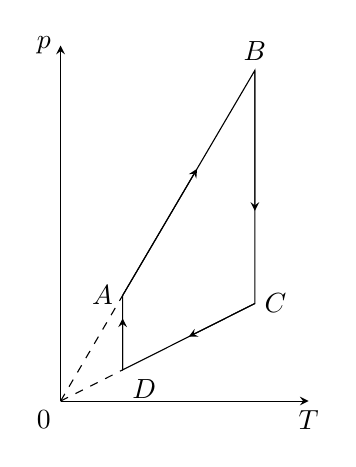
\begin{tikzpicture}[>=stealth,scale=1.05]
\draw[->] (0,0)--(3,0) node[below] {$T$};
\draw[->] (0,0)--(0,4.3) node[left] {$p$};
\node[below left] at (0,0) {$0$};
\coordinate (A) at (.75,{4*.75/2.35});
\coordinate (B) at (2.35,4.0);
\coordinate (C) at (2.35,1.18);
\coordinate (D) at (.75,{1.18*.75/2.35});
\draw[dashed] (0,0)--(A);
\draw[dashed] (0,0)--(D);
\draw (A)--(B)--(C)--(D)--cycle;
\draw[->] (A)--(1.65,{4*1.65/2.35});
\draw[->] (B)--(2.35,2.3);
\draw[->] (C)--(1.55,{1.18*1.55/2.35});
\draw[->] (D)--(.75,1.0);
\node[left] at (A) {$A$};
\node[above] at (B) {$B$};
\node[right] at (C) {$C$};
\node[below right] at (D) {$D$};
\end{tikzpicture}
\end{center}
На рисунке показан график циклического процесса, проведённого с одноатомным идеальным газом, в координатах $p$--$T$, где $p$ --- давление газа, $T$ --- абсолютная температура газа. Количество вещества газа постоянно.
\begin{enumerate}
\item Газ за цикл совершает положительную работу.
\item В процессе $AB$ газ получает положительное количество теплоты.
\item В процессе $BC$ внутренняя энергия газа уменьшается.
\item В процессе $CD$ над газом совершают работу внешние силы.
\item В процессе $DA$ газ изотермически расширяется.
\end{enumerate}
}{
\smallskip\noindent\textbf{Решение от GPT}\par
Из $pV=\nu RT$ следует, что $AB$ и $CD$ --- изохоры, причём $V_{AB}<V_{CD}$. Участки $BC$ и $DA$ --- изотермы, $T_{BC}>T_{DA}$.
\begin{enumerate}
\item Верно: работа за цикл $A_{\text{ц}}=\nu R(T_{BC}-T_{DA})\ln(V_{CD}/V_{AB})>0$.
\item Верно: на $AB$ температура растёт, работа равна нулю, поэтому $Q=\Delta U=\frac32\nu R\Delta T>0$.
\item Неверно: на $BC$ температура постоянна, поэтому $\Delta U=0$.
\item Неверно: на изохоре $CD$ работа равна нулю.
\item Неверно: на $DA$ давление растёт при постоянной температуре, следовательно, газ сжимается.
\end{enumerate}
\textbf{Ответ: 12.}
}

% Source 196De7: https://ege.fipi.ru/bank/questions.php?search=1&proj=BA1F39653304A5B041B656915DC36B38&qid=196De7
\BankTask{196De7}{
\begin{center}
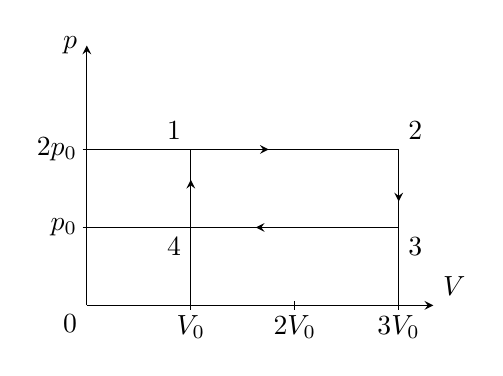
\begin{tikzpicture}[>=stealth,scale=1.1]
\draw[->] (0,0)--(4.0,0) node[above right] {$V$};
\draw[->] (0,0)--(0,3.0) node[left] {$p$};
\node[below left] at (0,0) {$0$};
\draw (0,.9)--(1.2,.9);
\draw (0,1.8)--(1.2,1.8);
\draw (1.2,0)--(1.2,.9);
\draw (3.6,0)--(3.6,.9);
\draw (1.2,.9)--(1.2,1.8)--(3.6,1.8)--(3.6,.9)--cycle;
\draw[->] (1.2,.9)--(1.2,1.45);
\draw[->] (1.2,1.8)--(2.1,1.8);
\draw[->] (3.6,1.8)--(3.6,1.2);
\draw[->] (3.6,.9)--(1.95,.9);
\foreach \x in {1.2,2.4,3.6}\draw (\x,-.05)--(\x,.05);
\foreach \y in {.9,1.8}\draw (-.05,\y)--(.05,\y);
\node[left] at (0,.9) {$p_0$};
\node[left] at (0,1.8) {$2p_0$};
\node[below] at (1.2,0) {$V_0$};
\node[below] at (2.4,0) {$2V_0$};
\node[below] at (3.6,0) {$3V_0$};
\node[above left] at (1.2,1.8) {$1$};
\node[above right] at (3.6,1.8) {$2$};
\node[below right] at (3.6,.9) {$3$};
\node[below left] at (1.2,.9) {$4$};
\end{tikzpicture}
\end{center}
Один моль аргона является рабочим телом в тепловом двигателе, который работает по циклу, показанному на рисунке в переменных $p$--$V$ ($p$ --- давление аргона, $V$ --- его объём).
\begin{enumerate}
\item Аргон получает положительное количество теплоты от нагревателя только в процессе $1$--$2$.
\item В процессе $3$--$4$ внутренняя энергия аргона не изменяется.
\item Работа аргона за цикл равна $2p_0V_0$.
\item В процессе $4$--$1$ аргон отдаёт холодильнику положительное количество теплоты.
\item Максимальная абсолютная температура аргона в цикле в $6$ раз больше минимальной.
\end{enumerate}
}{
\smallskip\noindent\textbf{Решение от GPT}\par
Для одного моля аргона $T=pV/R$, $U=\frac32RT$, $Q=\Delta U+A$.
\begin{enumerate}
\item Неверно: теплота поступает на $1$--$2$ и на $4$--$1$; в обоих процессах температура растёт.
\item Неверно: на $3$--$4$ произведение $pV$ уменьшается, поэтому $\Delta U<0$.
\item Верно: работа за цикл равна площади прямоугольника, $A_{\text{ц}}=(2p_0-p_0)(3V_0-V_0)=2p_0V_0$.
\item Неверно: на $4$--$1$ объём постоянен, температура растёт, поэтому $Q=\Delta U>0$.
\item Верно: максимальная температура достигается в точке $2$, минимальная --- в точке $4$; $T_2/T_4=(2p_0\cdot3V_0)/(p_0V_0)=6$.
\end{enumerate}
\textbf{Ответ: 35.}
}

% Source 0D668C: https://ege.fipi.ru/bank/questions.php?search=1&proj=BA1F39653304A5B041B656915DC36B38&qid=0D668C
\BankTask{0D668C}{
\begin{center}
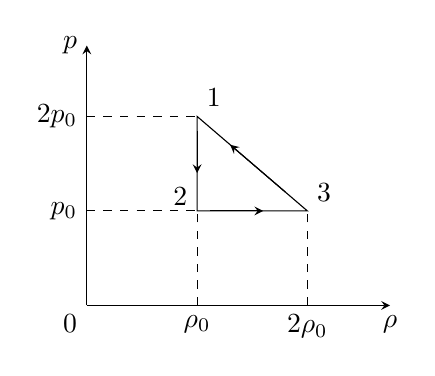
\begin{tikzpicture}[x=1.4cm,y=1.2cm,>=stealth]
\draw[->] (0,0)--(2.75,0) node[below] {$\rho$};
\draw[->] (0,0)--(0,2.75) node[left] {$p$};
\node[below left] at (0,0) {$0$};
\draw[dashed] (0,2)--(1,2);
\draw[dashed] (0,1)--(1,1);
\draw[dashed] (1,0)--(1,1);
\draw[dashed] (2,0)--(2,1);
\node[left] at (0,1) {$p_0$};
\node[left] at (0,2) {$2p_0$};
\node[below] at (1,0) {$\rho_0$};
\node[below] at (2,0) {$2\rho_0$};
\draw (1,2)--(1,1)--(2,1)--cycle;
\draw[->] (1,1.85)--(1,1.4);
\draw[->] (1.12,1)--(1.6,1);
\draw[->] (1.8,1.2)--(1.3,1.7);
\node[above right] at (1,2) {$1$};
\node[left] at (1,1.15) {$2$};
\node[above right] at (2,1) {$3$};
\end{tikzpicture}
\end{center}
\(1\,\text{моль}\) одноатомного идеального газа совершает цикл \(1-2-3-1\), при котором давление \(p\) газа изменяется с изменением плотности \(\rho\) газа так, как показано на рисунке. Значения плотности и давления в вершинах цикла представлены на графике.
\begin{enumerate}
\item Работа газа в процессе \(1-2\) равна нулю.
\item В процессе \(3-1\) газ отдаёт положительное количество теплоты.
\item Температура газа в состоянии \(3\) минимальна.
\item Внутренняя энергия газа в процессе \(2-3\) увеличивается.
\item При переходе газа из \(3\) в \(1\) внутренняя энергия не меняется.
\end{enumerate}
}{
\smallskip\noindent\textbf{Решение от GPT}\par
Для неизменной массы газа \(V=m/\rho\), \(T=Mp/(R\rho)\), где \(M\) — молярная масса. Обозначим \(T_0=Mp_0/(R\rho_0)\). Тогда
\[
T_1=2T_0,\qquad T_2=T_0,\qquad T_3=\frac{T_0}{2},\qquad U=\frac32\nu RT.
\]
1) Верно: \(\rho=\mathrm{const}\), следовательно, \(V=\mathrm{const}\) и \(A_{12}=0\).

2) Неверно: при переходе \(3\to1\) газ расширяется, \(A_{31}>0\), и нагревается, \(\Delta U_{31}>0\). Поэтому \(Q_{31}=\Delta U_{31}+A_{31}>0\): газ получает теплоту.

3) Верно: \(T_3<T_2<T_1\).

4) Неверно: \(T_3<T_2\), поэтому \(\Delta U_{23}<0\).

5) Неверно: \(T_1>T_3\), поэтому \(\Delta U_{31}>0\).

Ответ: \(13\).
}

\end{document}
